\documentclass{article}

\usepackage[ansinew]{inputenc}
\usepackage[spanish]{babel}
\usepackage[T1]{fontenc}
\usepackage{fancyhdr}
\usepackage{graphicx}
\usepackage[a4paper, total={6in, 8in}]{geometry}

\pagestyle{fancy}
\fancyhf{}
\rhead{Mart��n Romera Sobrado}
\chead{Dise�o del Software}
\lhead{PEC Febrero 2021}

\begin{document}
	\begin{titlepage}
		\centering
		\vspace*{1cm}
		
		\Huge
		\textbf{71013035 - Dise�o del Software}\\
		\textbf{2021}
		
		\vspace{0.5cm}
		\LARGE
		Centro Asociado de la UNED en Bizkaia\\
		Tutor: Aziz Mulud	
		\vspace{1.5cm}
		
		\textbf{Mart�n Romera Sobrado}\\
		\textbf{Bilbao}
		
		\vfill
		
		\vspace{0.8cm}
		\Large
		Horas de estudio de los contenidos hasta la fecha:\textbf{ 85 horas}\\
		
		Horas de dedicaci�n para realizar esta actividad:\textbf{ 20 horas}\\
		
		N�mero de actividades no evaluables realizadas:\textbf{ 22 actividades}\\
		 % TODO a�adir fecha
	\end{titlepage}
	\newpage
	\section{Cuestiones}
		\subsection{Fase de Inicio: Evaluaci�n de los Casos de Uso}
			\subsubsection{Casos de uso primarios}
				\textit{Represente en un diagrama UML de casos de uso, los casos de uso primarios (Elementary Business Process) m�s importantes, sus actores principales, los de apoyo y las interacciones correspondientes para el m�dulo SanGranja.}\\
				\begin{figure}[h]
					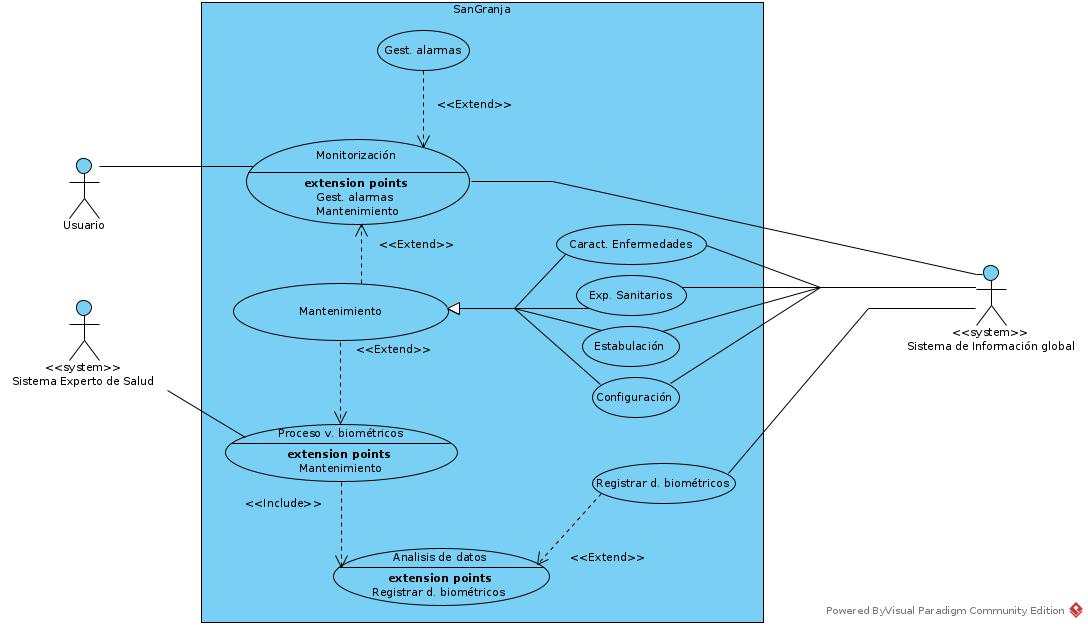
\includegraphics[width=\textwidth]{diagramas/CasosDeUsoPrimarios.jpg}
					\caption{Diagrama de Casos de Uso primarios.}
				\end{figure}
				
				
			\subsubsection{Caso de uso <<SimularPropagaci�nEnfermedad\_X>>}
				\textit{Con la siguiente descripci�n del caso de uso <<SimularPropagaci�nEnfermedad\_X>>, escribalo en un formato completo (se recomiendoa la variante ``en dos columnas'') y un estilo esencial (excluyendo los detalles t�cnicos de nivel bajo). Incluya tanto el flujo en el escenario principal de �xito como 2 extensiones o flujos alternativos que pudieran ser frecuentes:}\\
				\begin{table}[h!]
					\centering
					\begin{tabular}{|p{0.5\linewidth}|p{0.5\linewidth}|}
						\hline
						\textbf{Actor principal:} & \textit{Usuario} \\\hline
						\multicolumn{2}{|l|}{\textbf{Escenario pr�ncipal de �xito}} \\\hline
						\textit{Acci�n del actor} & \textit{Responsabilidad del Sistema} \\\hline
						1. El \textit{Usuario} establece en qu� \textit{Corrales} desea hacer la observaci�n. & 2. El \textit{Sistema} toma muestras de los datos biom�tricos de cada \textit{Corral} seleccionad \\
						& 3. El \textit{Sistema} realiza los c�lculos para estimar la previsi�n de la propagaci�n de la enfermedad en los corrales para un d�a. \\
						& \textit{El sistema repite el paso 3 para todos los d�as que haya establecido el usuario} \\
						& 4. El \textit{Sistema} presenta los resultados obtenidos de la iteraci�n del paso 3 en forma de una relaci�n bidimensional.\\\hline
						\multicolumn{2}{|l|}{\textbf{Escenario alternativo 1: El usuario interrumpe el proceso de c�lculos}}\\\hline
						\multicolumn{2}{|l|}{Pasos 1, 2 y 3 se mantienen de la misma manera}\\\hline
						4. El \textit{Usuario} decide interrumpir el proceso de c�lculo. & 5. El \textit{Sistema} realiza una petici�n de confirmaci�n al \textit{Usuario}\\
						6a El \textit{Usuario} acepta la petici�n & 7a El \textit{Sistema} desecha los c�lculos y vuelve al estado en el que se encontraba previo a la simulaci�n.\\
						6b El \textit{Usuario} no acepta la petici�n & 7b \textit{Sistema} reanuda los c�lculos y continua en el paso 3 del escenario principal.\\\hline
						\multicolumn{2}{|l|}{\textbf{Flujo alternativo 2: Alguno de los corrales no tiene animales enfermos}}\\\hline
						\multicolumn{2}{|l|}{Pasos 1 y 2 se mantienen de la misma manera}\\\hline
						& 3. El \textit{Sistema} detecta que hay un corral sin animales infectados\\
						& 4. El \textit{Sistema} elimina ese corral para los c�lculos de la simulaci�n\\
						& 5. El \textit{Sistema} reanuda los c�lculos y continua en el paso 3 del escenario principal.\\\hline
					\end{tabular}
					\caption{Caso de Uso <<SimularPropagaci�nEnfermedad\_X>>}
				\end{table}
		\subsection{Fase de Elaboraci�n: Modelado Conceptual}
			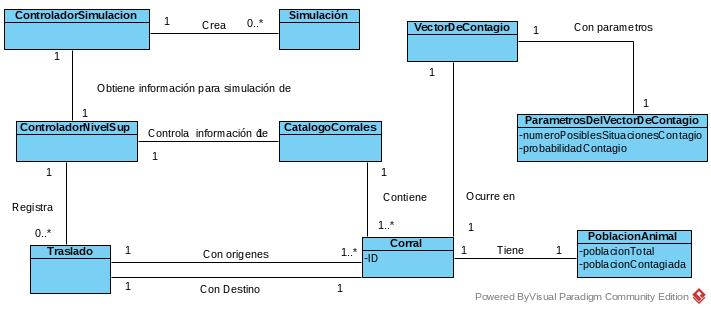
\includegraphics[width=\linewidth]{diagramas/MDom SimularPropagacionEnfermedad_X Clases Conceptuales.jpg}
			
\end{document}